%o   Project goal and motivation
%o   Project summary and overview - the "red thread"
%o   Project results (brief summary)
%o   Dissertation Layout
%
%Nytta med projektet, bakomliggande motivering, hypotes kring resultat (Google Glass kommer vara bättre än smartphone eftersom handsfree and stuff), layout av rapporten.
%
%Prata allmänt om vad det finns för problem idag, mer specifikt vad kommer vår applikation att lösa, mixa med frågor som kan besvaras bland slutsatserna
%
%
%

Although assembling components in to a fully functional product can be a tedious task and done by the books, step-by-step, an employee constructing many different products may not be able to learn the process by heart, and will need to rely on instruction manuals.

However, carrying instruction manuals around would mean having to find specific instruction and also, while assembling components, the instructions will have to be laid aside. As such, the constructor's focus will have to shift between the components and the instructions, perhaps turn the head around, and potentially the constructor may even need to use their hands in order to browse the instructions. 

Using a smartphone at least removes the requirement for written instructions on paper, but a smartphone still requires touch and as such will occupy at least one of the constructor's hands at some point. A smartphone, similar to ring binders, will also have to be laid aside.

One solution to the problem would be using a TV or computer screen. Controlled with for instance foot pedals the instructions could be browsed without using hands. However, such technology requires space and also comes with the fact that such technology is not very mobile. Screens and foot pedals would have to be positioned at specific locations. Considering a production line may have several stations screens and foot pedals would have to be placed at each one of them. Trying to assemble components outside of those stations would not be possible, provided that the instructions would be necessary.

New technology may offer a better solution. Google Glass is a computational device, which looks and is worn as regular glass frames~\cite{glassStart}. Google Glass also has a display positioned slightly above the user's line of sight, meaning that Google Glass does not have to be taken off and put down. Google Glass may also be entirely controlled via voice commands, meaning that the user may operate Google Glass completely hands free.

This dissertation describes the design, implementation and evaluation of an application for Google Glass. Using the application, user's will be able to scan a QR code related to a specific product and get information on which components are needed to construct the specific product, as well as instructions on how to assemble the components.

The application will also be built for smartphones, giving a reference point for the evaluation as well as a method of comparison with the Google Glass application. Using the Google Glass application users will be able to construct products by following instructions, but without having to shift their focus from what they are doing, and neither will the users have to use their hands in order to control the application.

The application, described in Figure~\ref{projectmapLightVersion}, will scan a QR code, download information based on the information received from the QR code, and the display the downloaded information in the form of a slide view. The application will exist in two versions, one for Google Glass and another for smartphones. However, the will both function the same and as such the device in Figure~\ref{projectmapLightVersion} can be either Google Glass or a smartphone.

	\begin{figure}[ht!]
		\centering
		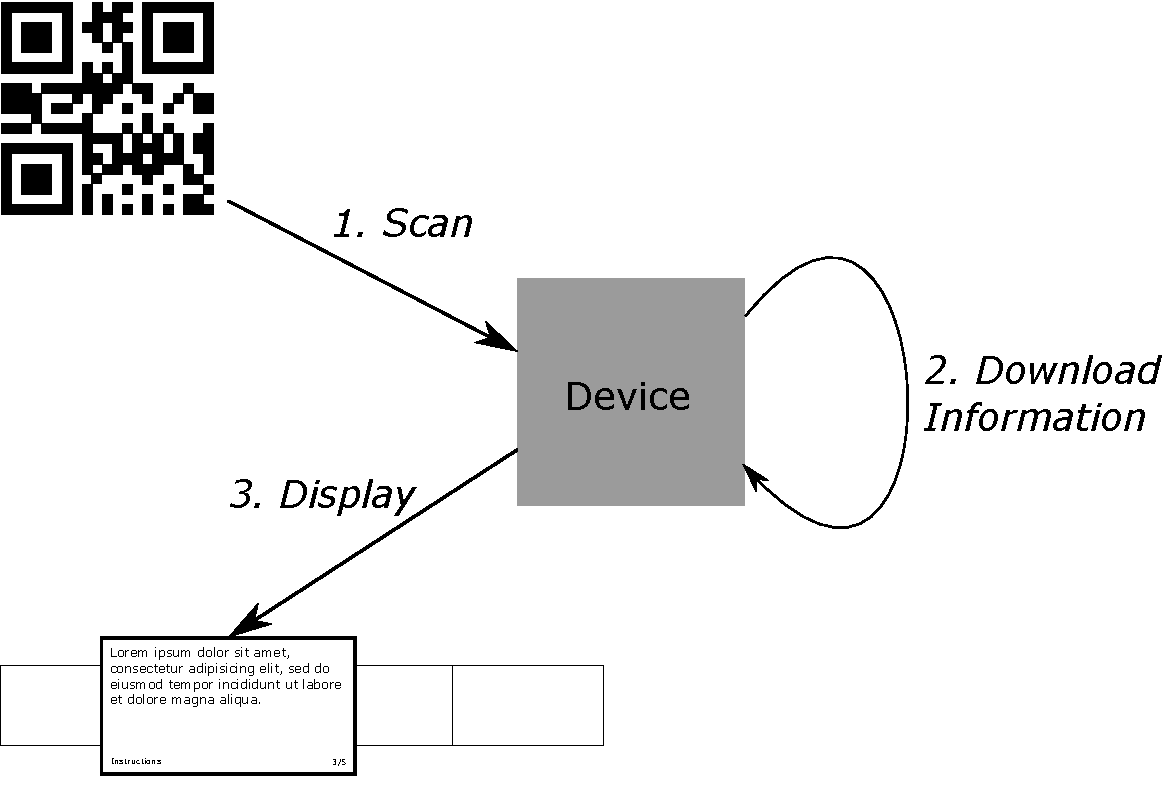
\includegraphics[width=110mm]{images/projectmapLightVersion}
		\caption{Application functionality.}
		\label{projectmapLightVersion}
	\end{figure}

\subsection{Discontinuance of the Explorer Program}
It should be noted that, since the start of this dissertation, Google have chosen to cancelled the so called ``explorer program'' for Google Glass~\cite{glassDiscontinued}. The explorer program was the ``open beta phase'' of Google Glass where Google, although Google Glass was sold as a consumer product, were still developing Google Glass at Google's research center, called Google X. Google used user's input and feedback to improve on Google Glass as a product, both in terms of hardware as well as software.

Coming out of the open beta phase, Google have now chosen to keep developing Google Glass, but without the help of consumers, meaning that any further updates, both in terms of hardware as well as software, will (as of now) not be publicly available. Google states that they are ``thrilled to be moving even more from concept to reality'', when discussing the future of Google Glass. As of January 20th, 2015, the Google Glass Explorer Edition was no longer available for sale. However, Google ensures that Google Glass will return ``when they're ready'', but does not go in to further details on when Google Glass will be available for sale again or what the new version will entail. 

\subsection{Back End}
The project has been divided in to two different parts. This dissertation will cover the front end part of the project, which includes building the applications, both the Google Glass version and the smartphone version. This dissertation will also discuss the different ways of presenting information and how information is presented in the application.

However, another part of the project is the back end part. The backend part has been summed up in Figure~\ref{projectmapLightVersion} as ``Download Information''. The back end part was done by Richard Hoorn and consists of web application programming interface (API), connected to a database in which all product information is stored. 

\subsection{Hypothesis}
The hypothesis is that the Google Glass application will prove useful and valuable, more so than the smartphone application. Although Google Glass might not be the most powerful device on the market, the features of Google Glass are the selling points. As such Google Glass could be deemed the better option over smartphones despite potentially worse results in comparison to smartphones. Google Glass is not expected to perform better than smartphones, but only to be reasonably behind smartphones, giving weight to the argument that Google Glass should be used in order to make the assembling of components an easier task. The difference in time should be such that the task to be performed does not take significantly longer to perform when using Google Glass in comparison to using a smartphone, taking in to account the hands free aspect of Google Glass.

Google Glass can also not be expected to fit the same amount of information on screen as smartphones, as the Google Glass screen is smaller than the screen on smartphones currently on the market. Similar to the time difference, the difference in the amount of information Google Glass si able to display, in comparison to smartphones, should be such that the necessary information would still be possible to get across to the user.

\subsection{Project Results}
The results show that Google Glass is almost always slower, both in terms of decoding the QR code and presenting the information to the user. On average Google Glass is about half a second slower than smartphone equivalents. In terms of the amount of information that may be displayed on the Google Glass display compared to the display on smartphones it was shown that the same amount of text that filled the screen on a smartphone needed three to four separate screens on Google Glass.

\subsection{Dissertation Layout}
Chapter~\ref{sec:background} discuss relevant background information regarding Google Glass. The chapter will include an introduction to what Google Glass is, how they came about and what features they have. The background chapter will also discuss similar products to Google Glass, as well as compare Google Glass to smartphones. Finally chapter two will include some discussion on topics relevant to the project, including QR code and ways of presenting information.

Chapter~\ref{sec:design} is about the design of the project. The discussion revolves around how the application is intended to work, and what limitations may apply to the implementation of the application, both on Google Glass and smartphone. The third chapter also discusses the design of the tests done on the application.

Chapter~\ref{sec:implementation} describes the implementation part of the project. The flow of the application is described in detail. Specific aspect of the application is also described in more detail. The layout of the slides as well as the voice commands. The experimental setup and how the tests were performed is also described here.

In chapter~\ref{sec:resultevaluation} the results of the tests are presented. The results are presented along with comments regarding how the results are to be interpreted as well as comments on any potential error factors during testing.

The final chapter, chapter~\ref{sec:conclusion}, contains conclusions on the project. The conclusions regards the test results, as well as conclusions on the project as a whole. Chapter six also includes comments based on personal user experience from using Google Glass for about three months. Finally future work is discussed and the report is concluded with some concluding remarks.

Attached to the dissertation, after the reference list, are appendices. In appendix~\ref{sec:abbreviations} abbreviations used throughout the dissertation are listed. Appendix~\ref{app:results} shows all the individual test results. Project code can be found in appendix~\ref{app:code}. Appendix~\ref{app:projectspec} is the last appendix which contains the original project specification, written in Swedish.